\documentclass[Report.tex]{subfiles}
\begin{document}
\newpage
\chapter{Appendix}
\setcounter{page}{1}
\setcounter{table}{0}
\setcounter{figure}{0}
\setcounter{section}{0}
\renewcommand{\thetable}{A\arabic{table}}
\renewcommand{\thefigure}{A\arabic{figure}}

\begin{longtable}{| p{0.9\textwidth} |}\hline
\textbf{Vocabulary Name}\\ \hline
AI/RHEUM\\
Alcohol and Other Drug Thesaurus\\
Authorized Osteopathic Thesaurus\\
Anatomical Therapeutic Chemical Classification System\\
Clinical Classifications Software\\
Consumer Health Vocabulary\\
COSTAR\\
CRISP Thesaurus\\
COSTART\\
Vaccines Administered\\
DXplain\\
Foundational Model of Anatomy Ontology\\
Gene Ontology\\
Healthcare Common Procedure Coding System\\
HUGO Gene Nomenclature Committee\\
HL7 Vocabulary Version 2.5\\
HL7 Vocabulary Version 3.0\\
ICD-10-PCS\\
International Classification of Diseases\\
International Classification of Primary Care\\
Library of Congress Subject Headings\\
Library of Congress Subject Headings, Northwestern University subset\\
LOINC\\
McMaster University Epidemiology Terms\\
MedlinePlus Health Topics\\
Medical Subject Headings\\
UMLS MetaThesaurus\\
MetaThesaurus CMS Formulary Reference File\\
MetaThesaurus FDA National Drug Code Directory\\
MetaThesaurus FDA Structured Product Labels\\
MetaThesaurus HCPCS Hierarchical Terms\\
Minimal Standard Terminology (UMLS)\\
NCBI Taxonomy\\
NCI Thesaurus\\
Biomedical Research Integrated Domain Group Model\\
BioCarta online maps of molecular pathways, adapted for NCI use\\
U.S. Centers for Disease Control and Prevention\\
Clinical Data Interchange Standards Consortium\\
Cancer Research Center of Hawaii Nutrition Terminology\\
Common Terminology Criteria for Adverse Events\\
Cancer Therapy Evaluation Program - Simple Disease Classification\\
NCI Division of Cancer Prevention Program\\
Digital Imagining Communications in Medicine\\
NCI Developmental Therapeutics Program\\
U.S. Food and Drug Administration\\
International Conference on Harmonization\\
Jackson Laboratories Mouse Terminology, adapted for NCI use\\
KEGG Pathway Database\\
NCI Dictionary of Cancer Terms\\
NCI Health Level 7\\
National Council for Prescription Drug Programs\\
National Institute of Child Health and Human Development\\
National Cancer Institute Nature Pathway Interaction Database\\
Registry Nomenclature Information System\\
Unified Code for Units of Measure\\
Zebrafish Model Organism Database\\
NCI SEER ICD Neoplasm Code Mappings\\
National Drug File\\
National Drug File - FDASPL\\
National Drug File - FMTSME\\
Online Mendelian Inheritance in Man\\
Physician Data Query\\
Quick Medical Reference (QMR)\\
QMR clinically related terms from Randolph A. Miller\\
RxNorm Vocabulary\\
Source of Payment Typology\\
Standard Product Nomenclature\\
USP Model Guidelines\\
University of Washington Digital Anatomist\\
National Drug File\\ \hline
\caption{List of vocabularies included in the MetaThesaurus subset. Full information on each can be found at \url{http://www.nlm.nih.gov/research/umls/sourcereleasedocs/index.html}.\label{tab:vocabs}}
\end{longtable}
\newpage

\lstset{frame=tb,
  language=SQL,
  aboveskip=3mm,
  belowskip=3mm,
  showstringspaces=false,
  columns=flexible,
  basicstyle={\small\ttfamily},
  numbers=none,
  numberstyle=\tiny\color{gray},
  keywordstyle=\color{blue},
  commentstyle=\color{dkgreen},
  stringstyle=\color{mauve},
  breaklines=true,
  breakatwhitespace=true,
  tabsize=3
}

\noindent Listing 2: SQL query used in \texttt{umls.py} to retrieve Semantic Type and direct parent of all concepts
\begin{lstlisting}
SELECT * FROM (
	SELECT S.CUI AS CHILD_CUI, M0.CUI2 AS PARENT_CUI, C0.STR AS PARENT_STR, S.STY AS S_TYPE
	FROM MRSTY AS S
	LEFT OUTER JOIN MRREL AS M0 ON M0.CUI1 = S.CUIAND M0.RELA='inverse_isa'
	LEFT OUTER JOIN MRCONSO AS C0 ON C0.CUI = M0.CUI2 AND C0.STT='PF' AND C0.ISPREF='Y'
	LEFT OUTER JOIN MRRANK AS R0 ON (C0.SAB = R0.SAB AND C0.TTY = R0.TTY)
	WHERE S.CUI IN (CUI_LIST)
	ORDER BY R0.RANK DESC, PARENT_CUI ASC, S.STN ASC) AS TT
GROUP BY TT.CHILD_CUI
\end{lstlisting}
\newpage

\begin{table}[ht!]
\begin{center}
    \begin{tabular}{ | l | c | c | }\hline
    \textbf{Country} & \textbf{Papers (\%)} & \textbf{Papers in} \\
     & &\textbf{dataset}\\ \hline
    USA & 28.1 & 14\\ \hline
    China & 8.5 & 4\\ \hline
    United Kingdom & 7.7 & 4\\ \hline
    Japan & 5.8 & 3\\ \hline
    Germany & 5.1 & 3\\ \hline
    Italy & 3.7 & 2\\ \hline
    Canada & 3.5 & 2\\ \hline
    France & 3.5 & 2\\ \hline
    Australia & 2.6 & 1\\ \hline
    India & 2.6 & 1\\ \hline
    \end{tabular}
    \caption{Percentage share of published papers between 2008 and 2012 for the 10 countries with the highest values.\label{tab:countries}}
\end{center}
\end{table}

\begin{table}[ht!]
    \begin{tabular}{| l |}\hline
26313663\\
26313665\\
26313747\\
26313755\\
26313765\\
26313805\\
26313850\\
26313852\\
26313854\\
26313868\\
26313870\\
\textbf{26313874}\\
26313875\\
26313888\\
26313894\\
26313898\\
26313900\\
26313901\\
26313902\\
\textbf{26313905}\\
26313916\\
26313935\\
26314029\\
26314035\\
\textbf{26314039}\\
26314069\\
\textbf{26314071}\\
\textbf{26314072}\\
\textbf{26314080}\\
\textbf{26314082}\\
\textbf{26314084}\\
\textbf{26314086}\\
\textbf{26314087}\\ \hline
\end{tabular}
\caption{List of PubMed IDs of papers used for assessing geocoding hit rate and accuracy. Accuracy papers were a subset of hit rate papers - emboldened IDs were used in both.\label{tab:dataset}} 
\end{table}

\begin{figure}[!ht]
\begin{center}
	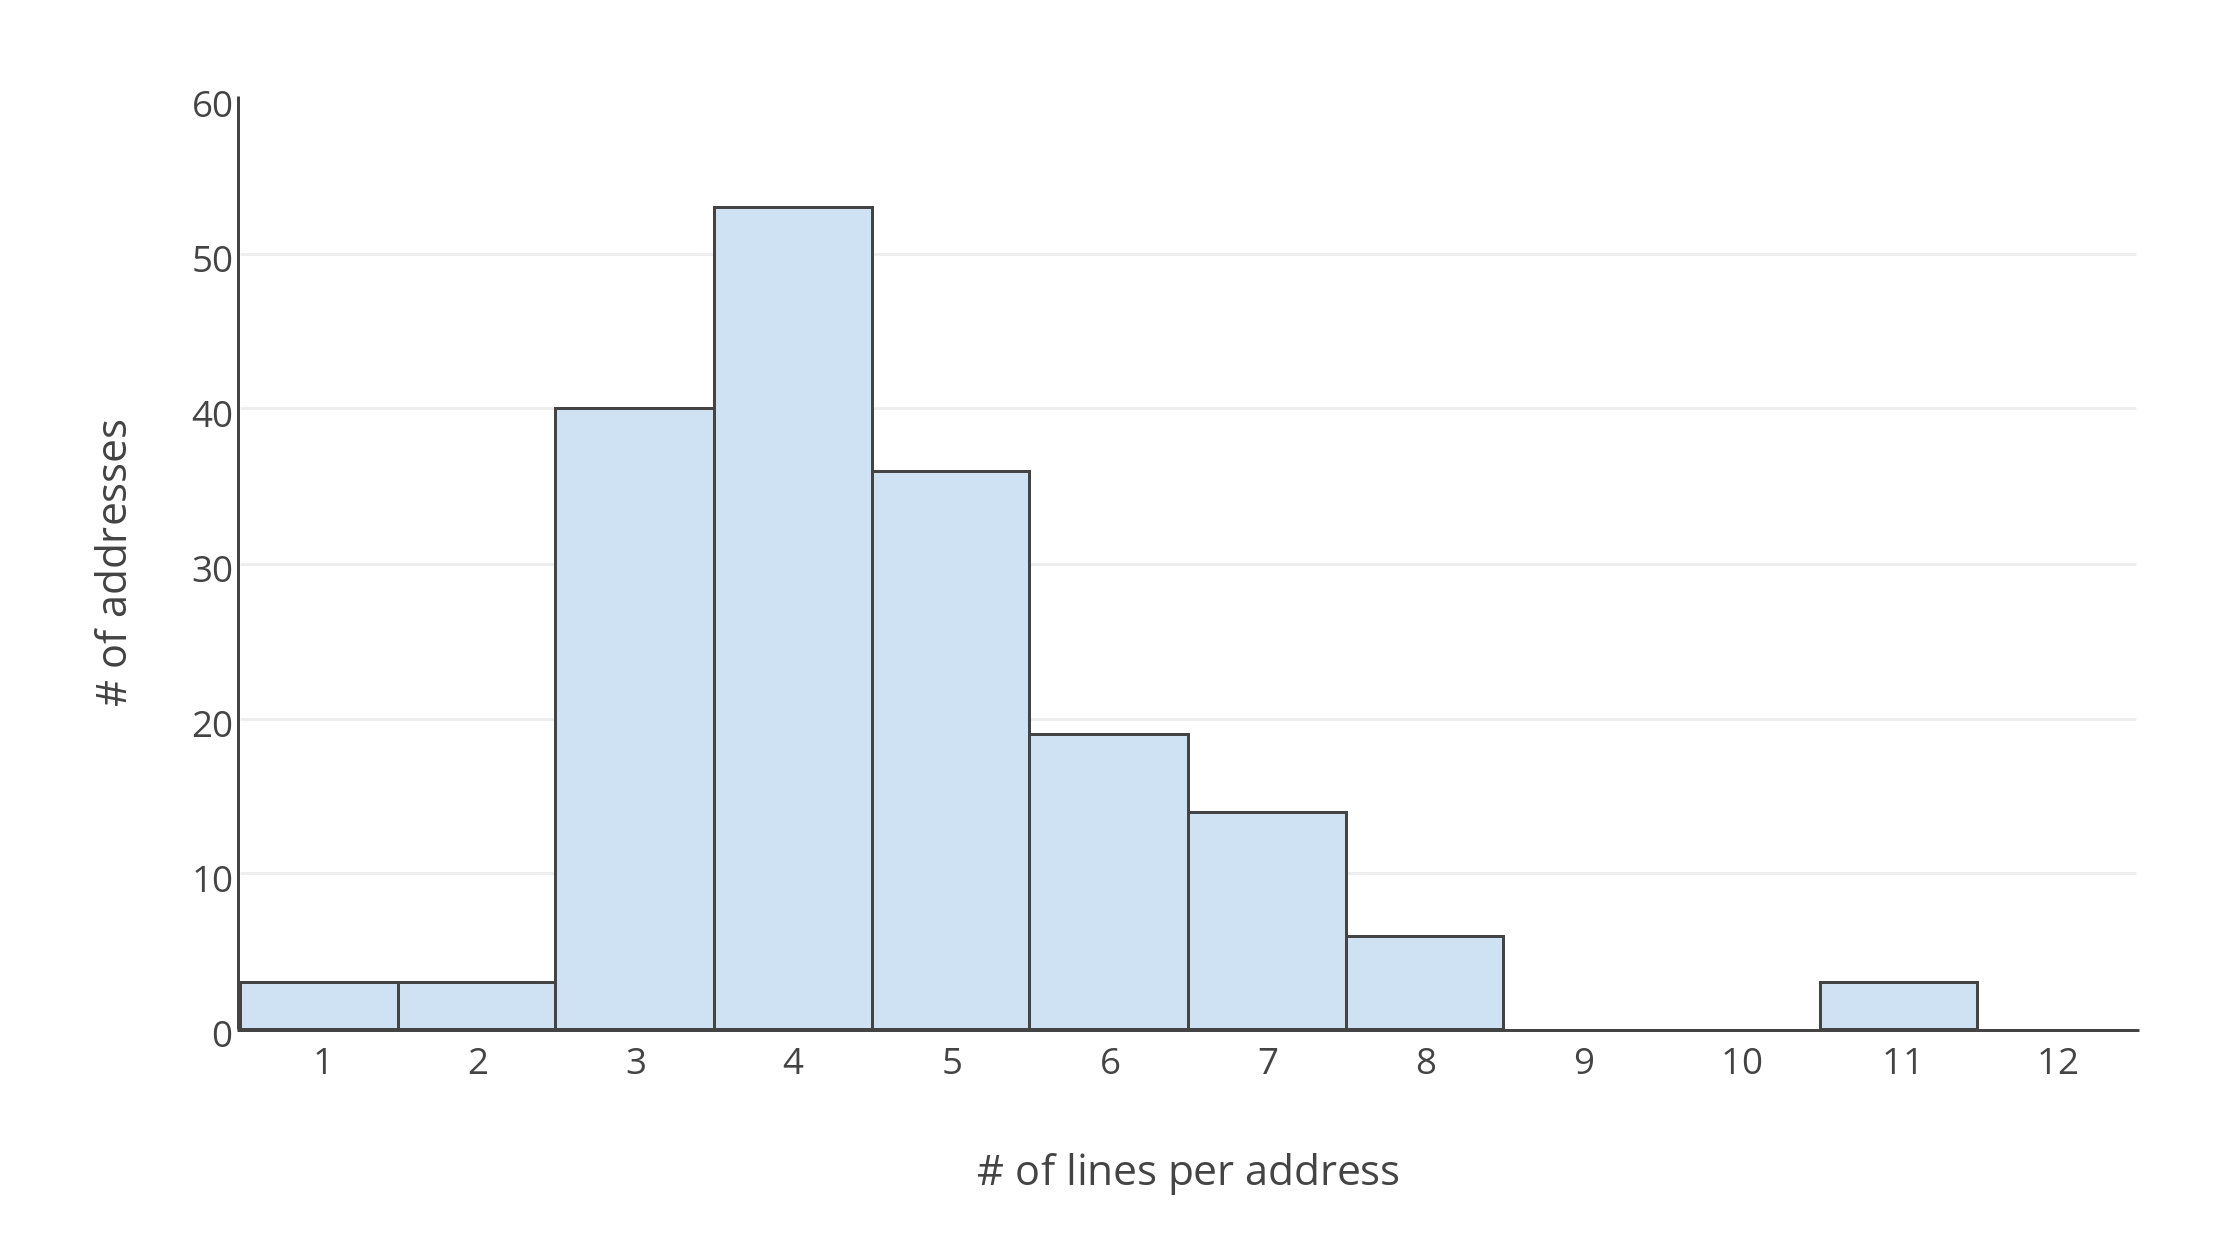
\includegraphics[width=0.8\textwidth]{../lib/images/address-lines-histogram}\\
	\caption{A histogram of the number of lines found in 178 addresses.\label{fig:addresslines}}
\end{center}
\end{figure}

\noindent Listing 3: Example of a log file, detailing the results of a search.
\begin{verbatim}
Search term: computer
0 documents retrieved from database.
1 documents fetched from PubMed.
Formatted address (format0): Orthopaedics and Traumatology Clinic, 
Taksim Training and Research Hospital, Istanbul, Turkey.
Formatted address (format0): Health Sciences Faculty, Istanbul University, 
Istanbul, Turkey.
Formatted address (format1): Taksim Training and Research Hospital, 
Istanbul, Turkey.
Output address: Witt Istanbul Suites
Coordinates: 41.029124, 28.982039
Formatted address (format1): Istanbul University, Istanbul, Turkey.
Output address: Istanbul University
Coordinates: 41.012604, 28.961838

24804813:
	9 concepts.
		['Computer Literacy', 'C0009603']
		['Cross-Sectional Studies', 'C0010362']
		['Nurse', 'C0028661']
		['Attitude to Computers', 'C0004273']
		['Computers', 'C0009622']
		['Nursing Staff, Hospital', 'C0028699']
		['Attitude of Health Personnel', 'C0004272']
		['Hospitals, University', 'C0020028']
		['Questionnaires', 'C0034394']
	2 place IDs.
		ChIJl2rUtNi5yhQR7unQJ246G3c
		ChIJ42s83I25yhQRemLN24uSUU8
1 inserted:
55f498df8da009211733a1ed
\end{verbatim}\\

\end{document}